\begin{frame}{Experiments}
\begin{center}
\textcolor{red}{How well does Q estimate the true returns?}
\end{center}
\begin{figure}
    \centering
    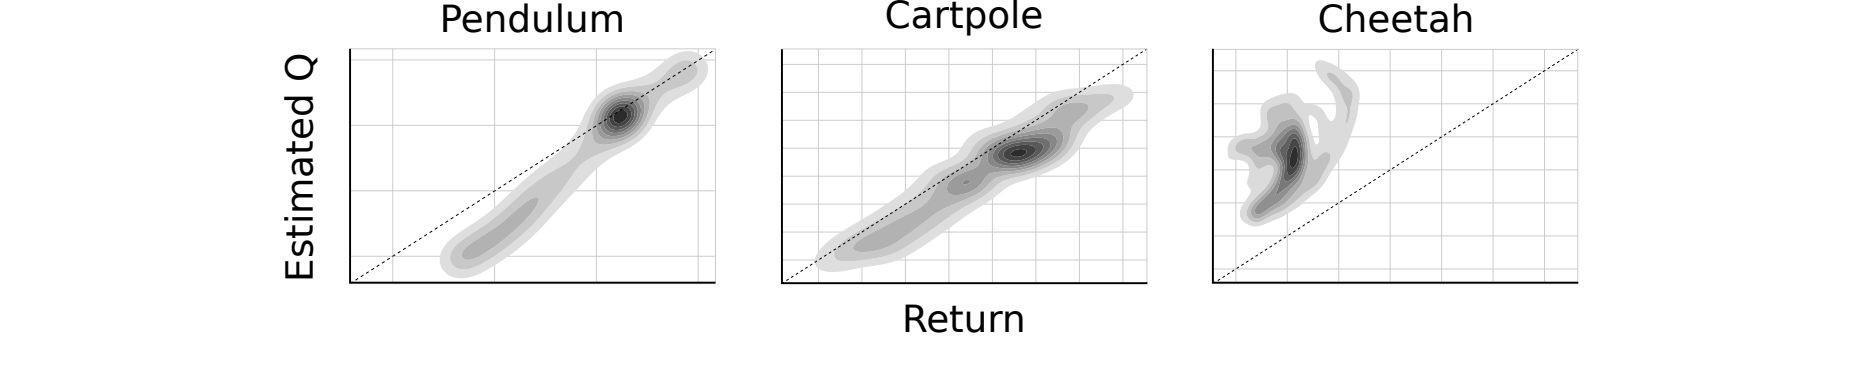
\includegraphics[width=0.85\textwidth,height=0.55\textheight,keepaspectratio]{images/continuous-control-1/figures/q-estimate-density-plots.jpg}
    \caption*{\footnotesize Figure 3: Density plot showing estimated Q values versus observed returns sampled from test episodes on 5 replicas. In simple domains such as pendulum and cartpole the Q values are quite accurate. In more complex tasks, the Q estimates are less accurate, but can still be used to learn competent policies. Dotted line indicates unity, units are arbitrary. (Figure: DDPG \rref{5}.)}
\end{figure}
\end{frame}
